\documentclass[a4paper]{article}

\usepackage{amsmath}
\usepackage{enumitem}

\usepackage{caption}

\usepackage{subfigure}
\usepackage{amsmath, amssymb}
\usepackage{graphicx}
\author{Kennard Ng and Luo Wen Han}
\title{Project 1: Manhattan World}

\bibliographystyle{unsrt}

\begin{document}
	\maketitle
	\section{Introduction}
	
	In this project, we use the expectation maximization framework to simultaneously obtain the extrinsic camera parameters i.e. the camera's rotation matrix and its translation, and the vanishing points of the image. 
	
	This problem is a chicken-and-egg problem where the camera rotation is needed to determine the vanishing points, and the vanishing points can be used to determine the camera rotation. 
	
	We apply the expectation maximization framework to images that are consistent with the Manhattan World Assumption to simultaneously obtain the extrinsic camera parameters and the vanishing points in the image. Under the Manhattan World Assumption, the camera rotation is obtained when the camera aligns itself with the natural Cartesian grid of the world coordinate. 
	
	\section{Background}
	
	\subsection{Vanishing Points}
	
	Under perspective projection, parallel lines in the 3D world appears to converge in images e.g. Figure \ref{fig:vp_eg}.
	
	\begin{figure}[ht]
		\centering
		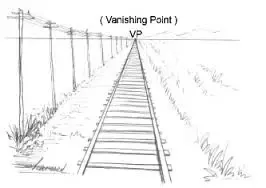
\includegraphics[width=0.5\linewidth]{images/vp_eg}
		\caption{Vanishing Point Example}
		\label{fig:vp_eg}
	\end{figure}

	The point of convergence is known as the vanishing point with lines in the image pointing towards the vanishing point being described as vanishing lines. We derive the vanishing point in the image from the homogeneous vanishing point $V$, rotation matrix $R$ and camera intrinsics $K$: 
	
	\begin{equation}
		v = K \times R \times V
	\end{equation}
	
	and take the cross-product of the vanishing point vector and the homogeneous pixel coordinate $u$ to determine the true orientation of the pixel $\theta_p$.
	
	
	\section{Our Approach}
	
	In our approach, we define the rotation matrix by its euler angles: $\alpha$, $\beta$ and $\gamma$. $\alpha, \beta$ and $\gamma$ are the rotation angles about the $x, y$ and $z$ axes respectively. We let $\Psi = (\alpha, \beta, \gamma)$.
	
	Given that the EM approach is sensitive to its initialization, we use the coarse-to-fine search strategy proposed in~\cite{Coughlan:2000:MWA:3008751.3008869} to obtain a good initial estimate. 
	
	\subsection{Initialization}
	
	We use the coarse-to-fine search strategy proposed in~\cite{Coughlan:2000:MWA:3008751.3008869} to initialize Euler angles before performing expectation minimization. In this search strategy, we explore discrete values to obtain a rough estimate of the camera parameters. From the search, we select the values that maximize the posterior over the search range:
	
	\begin{equation}
		P\left(M | G, \Psi\right) \propto P\left(G | M, \Psi\right) P(M),
	\end{equation}
	
	where $M, G$ and $\Psi$ denotes the assignment of pixels to vanishing points, the gradients of the pixels, and the Euler angles respectively. The likelihood $P\left(G | M, \Psi \right)$ is given by: 
	\begin{equation}
	P\left(G | M, \Psi \right)=\left\{\begin{array}{ll}\mathcal{N}(\Phi - \Theta |0, 0.5) & {\text { if } m = \{1, 2, 3\}} \\ {1 / 2\pi} & {\text { if } m=4}\end{array}\right.
	\end{equation}
	
	where $\Phi, \Theta$ is the estimated and the true orientation of the edge respectively, and $m=\{1,2,3\}$ denotes the assignment to vanishing points from the natural Cartesian grid of the image and $m={4}$ denotes an assignment to other vanishing points present in the image. Given that we wish to maximize the posterior across all pixels $p$, we find Euler angles that maximize the following:
	\begin{equation}
		\Psi^*=\underset{\Psi}{\operatorname{argmax}} \prod_p P(G_p|M,\Psi)P(M) = \underset{\Psi}{\operatorname{argmax}} \prod_{p} \sum_{m=1}^4 P\left(G_p|m, \Psi\right)p(m)
	\end{equation}
	
	Computing $\Psi^*$ using the above approach is computationally intractable since $\prod_p P(G_p|M,\Psi)P(M) \rightarrow 0$ as $p$ increases. Hence, we use the log trick to make it tractable and compute $\Psi^*$ as follows:
	
	\begin{equation}
		\Psi^{*}=\underset{\Psi}{\operatorname{argmax}} \sum_{p} \log\left\{\sum_{m=1}^{4} P\left(G_{p} | m, \Psi\right) p(m)\right\}
	\end{equation}
	
	The coarse-to-fine search begins with a coarse search for $\beta$ over the range $-\pi / 3$ to $\pi / 3$ at increments of $\pi / 90$, with $\alpha, \gamma = 0$. The result of the coarse search if the optimal coarse search value $\beta_c$.
	
	Then, a fine search is performed over $\alpha, \beta_c, \gamma$. Specifically, we explore over small permutations of $\pi / 90$ from $\beta_c$ for $\beta$,  $\pi / 36$ from $0$ for $\alpha$ and $\gamma$. By searching through the above values, we obtain a decent estimate of $\Psi$ as visualized in Figure~\ref{fig:initial_vp}.
	
	\begin{figure}[ht]
		\centering
		\begin{subfigure}
			\centering
			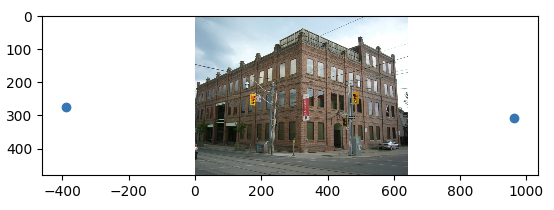
\includegraphics[width=0.9\columnwidth]{images/vp_init1.png}
		\end{subfigure}
		\begin{subfigure}
			\centering
			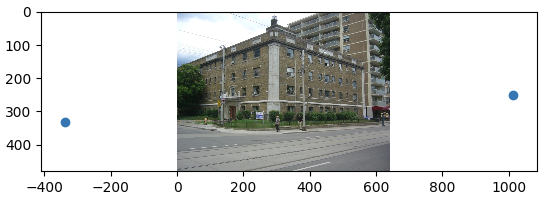
\includegraphics[width=0.9\columnwidth]{images/vp_init2.png}
		\end{subfigure}
		\caption{\label{fig:initial_vp}Initial Vanishing Point Estimates from~\cite{Coughlan:2000:MWA:3008751.3008869}.}
	\end{figure}
	
	However, because the search is performed discrete values, there is a loss of resolution, where $\Psi^*$ is not optimal but a coarse estimate. We further optimize $\Psi$ to be optimal in the Expectation Maximization (EM) framework as proposed in~\cite{atlanta-world}.
	
	\subsection{Expectation Maximization}
	
	In the E-step, we compute the soft assignment of each pixel $p$ to the models $m \in \{1, 2, 3, 4\}$. We define $w_{pm}$ to be the soft assignment for pixel $p$ to model $m$ i.e. vanishing point, computed as the normalized posterior with $\sum_m w_{pm}$ as the normalizer:
	
	\begin{equation}
		w_{pm} = \frac{P\left(G_{p} | m, \Psi^\text{old}\right)}{\sum_{m=1}^{4} P\left(G_{p} | m, \Psi^\text{old}\right) p(m)}
	\end{equation}
	
	where $\Psi^\text{old}$ is the Euler angle estimate from the previous M-step. We use $w_{pm}$ to update $\Psi$:
	
	\begin{equation}
		\Psi^\text{new}=\underset{\Psi}{\operatorname{argmax}} Q\left(\Psi ; \Psi^\text{old}\right).
	\end{equation}
	
	\begin{equation}
	\begin{aligned}
	Q\left(\Psi ; \Psi^\text{old}\right) &\triangleq \langle\log P(G | M, f(\Psi))\rangle+\log P(\Psi) \\
	&= \sum_{p}\left\langle\log P\left(\phi_{p} | m_{p}, f(\Psi)\right)\right\rangle+\log P(\Psi) \\
	&= \sum_{p} \sum_{m} w_{p m} \log P\left(\phi_{p} | m, f(\Psi)\right)+\log P(\Psi) \\
	&= \sum_{p} \sum_{m \in\{1, 2, 3\}} w_{p m}\left(\phi_{p}-\theta\left(f_{m}(\Psi), u_{p}\right)\right)^{2}+\log P(\Psi)
	\end{aligned}
	\end{equation}
	
	We optimize the final term of the M-step equation using least squares optimization where the residual for optimization is \(\sqrt{w_{pm}} \left(\phi_p - \theta(f_m(\Psi), u_p)\right)\), where $f(\Psi)$ is the vanishing points computed from the Euler angles $\Psi$, $u_p$ is the homogeneous coordinate of $p$, and $\theta(\cdot)$ is the true edge orientation. Essentially, we are minimizing the error between the true and estimated orientation $\phi_p$ for each pixel weighted by $w_{pm}$. We set $\log{P(\Phi)} = 0$ since there is no known prior. The final results are presented below: 
	\begin{figure}[ht]
		\centering
		\begin{subfigure}
			\centering
			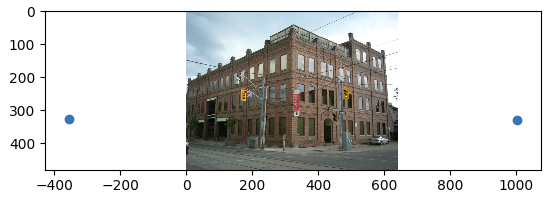
\includegraphics[width=0.9\columnwidth]{images/vp_final1}
		\end{subfigure}
		\begin{subfigure}
			\centering
			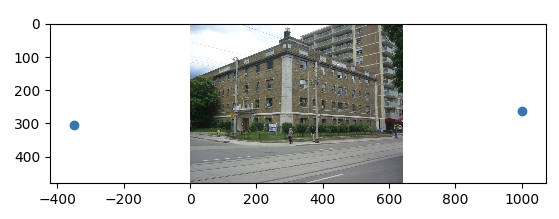
\includegraphics[width=0.9\columnwidth]{images/vp_final2}
		\end{subfigure}
		\caption{Final Vanishing Points Estimate}
	\end{figure}
	
	\begin{figure}[ht]
		\centering
		\begin{subfigure}
			\centering
			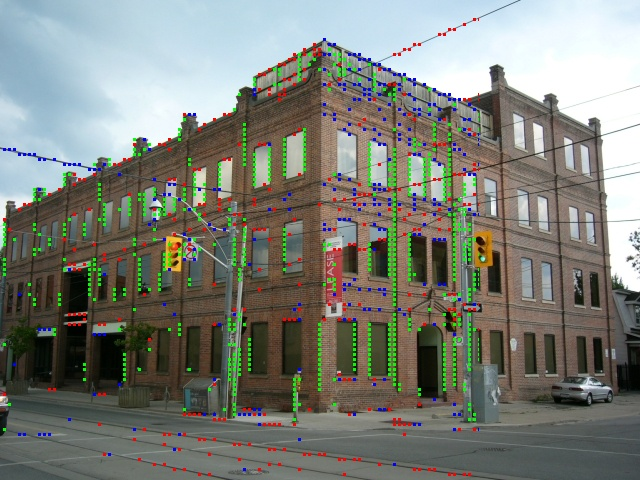
\includegraphics[width=0.9\columnwidth]{images/assignment1.jpg}
		\end{subfigure}
		\begin{subfigure}
			\centering
			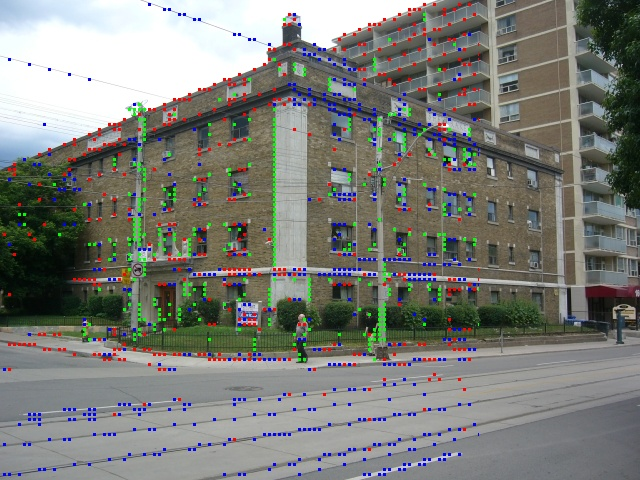
\includegraphics[width=0.9\columnwidth]{images/assignment2.jpg}
		\end{subfigure}
		\caption{Pixel Assignment.}
	\end{figure}

	\clearpage
	\bibliography{references.bib}
	
\end{document}